\section{Contribution}

\subsection{Visualization of the State Space}

\begin{figure}[h!]
\centering
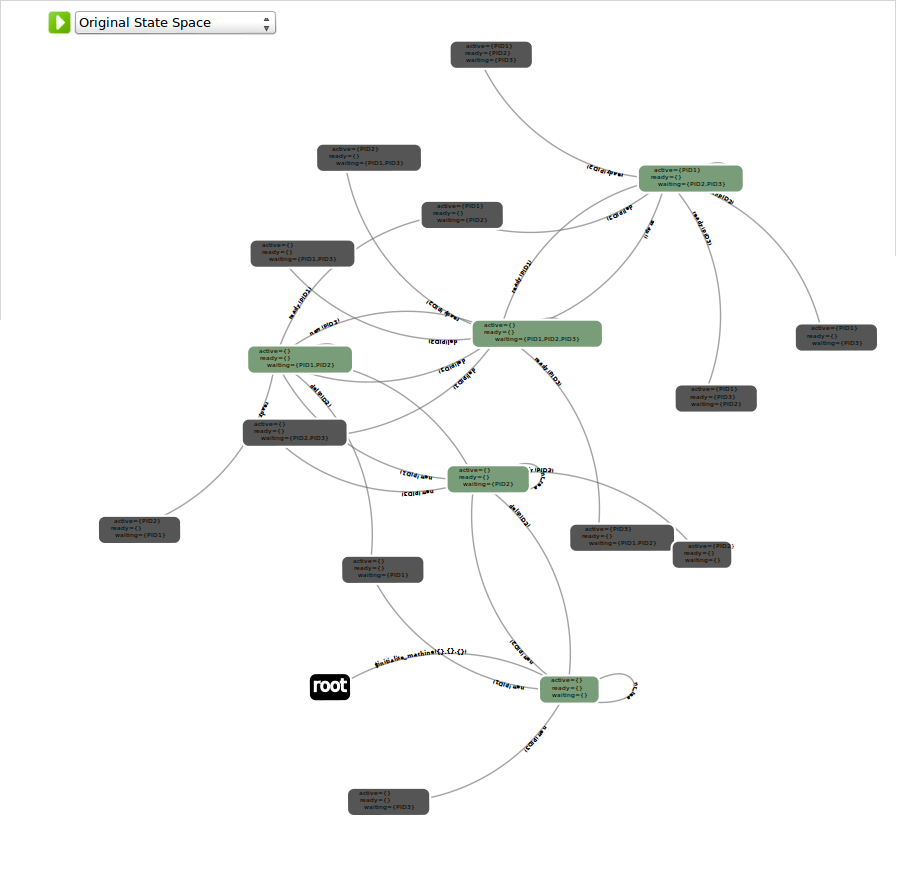
\includegraphics[width=15cm]{bilder/ss-zoomedOut.png}
\caption{Visualization of the state space for the Scheduler example}
\label{zoomedOut}
\end{figure}

When a state space visualization is opened, the visualization servlet responsible for the state space visualization takes the state space associated with the current animation and extracts the information about the nodes and edges contained within the graph. This information is then processed by D3 using the force layout. As a basis for the visualization, we used the Force Directed Graph example created by Michael Bostock (\ref{appendix:force}). Unfortunately, the state space contains an extremely large amount of information that has to be processed. This includes:

\begin{enumerate}
\item{How the state space graph appears as a whole.}
\item{The values of the variables for every state in the graph.}
\item{The names and parameters of the operation the corresponds with every edge in the graph.}
\item{The value of the invariant for every state in the graph.}
\item{Whether or not a given node within the graph is deadlocked.}
\item{Multiple edges between given states.}
\item{Looped edges to one given state.}
\item{The direction of any given edge.}
\item{A special representation to show the root node within the graph.}
\end{enumerate}

Because of all of these things, it was rather difficult to create a useful visualization of the whole state space because the user not only wants to inspect how the state space appears as a whole but also the individual states within the operation. To solve this problem, we used the zoom functionality that is available in D3. The main problem was that if the visualization of the nodes was large enough for the user to read the values of the variable at the given state, it would no longer be possible to see the state space as a whole. Instead of trying to meet both requirements at once, we simply made the text that is printed on the node and edge objects very small. When the visualization is created, the user can inspect the graph as a whole how the graph appears as a whole. The text for the given nodes, however, is virtually indiscernable. If the user wants to inspect a particular node, they can do so by zooming into the visualization. The text is then larger, and the user can see the nodes that are in the direct neighborhood of the node in question. Then user can also click on the background of the visualization in order to pan through the visualization and inspect other nodes and edges. The visualization is interactive. The user can grab a node and move it around to a desired position.

\begin{figure}[h!]
\centering
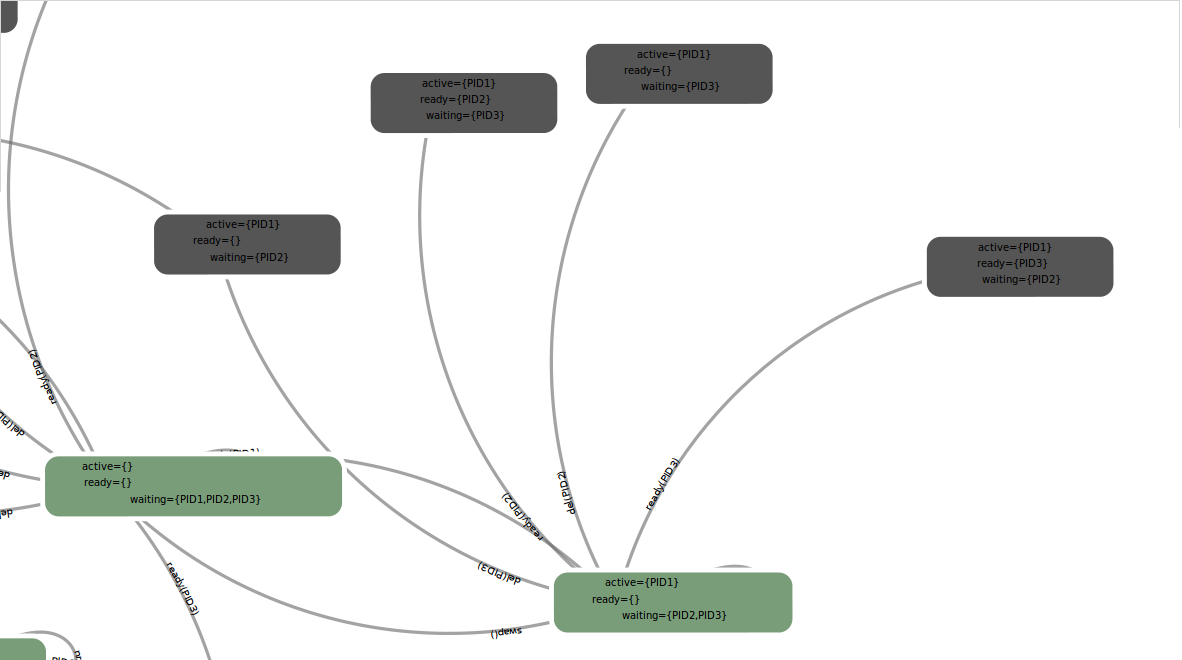
\includegraphics[width=15cm]{bilder/ss-neighborhood.png}
\caption{Visualization of the neighborhood of a state in the state space visualization}
\label{neighborhood}
\end{figure}

The visualization of the edges was also not trivial. For most implementations of the force layout, developers use lines as edges. The problem with lines is that if multiple edges occur between two nodes (which happens almost always in a state space), the edges within the representation will be drawn on top of each other. To avoid this, it was necessary to use the SVG path object instead of the SVG line object. Then the paths are drawn with a curve and they do not appear on top of each other. It was also necessary to find a way to determine how many edges exist between two nodes, because if the arcs are generated statically, there is still a good possibility that they will be drawn on top of each other. In order to do this, we identified and numbered multiple edges and self-loops. Then the edges and loops can be drawn and adjusted so that they are not drawn on top of each other.

We also had some performance issues that were associated with very large state spaces. The force layout keeps adjusting the graph until it reaches a fix point. The problem was that as the state space grew, there were more and more objectst that had to be accounted for. The force layout just kept calculating and moving the the nodes. This didn't only affect the appearance of the visualization. It cost enough resources that the whole eclipse plugin would become unresponsive. A quick fix to this problem was adding a play/pause button to the upper left hand corner of the visualization. When the user is satisfied with the visualization and how it is laid out, he can press the pause button, and the graph will stop being rendered. When he presses the play button, the rendering will begin again. The iterative force layout keeps running in the background, so when the rendering begins again, the visualization has had time to stabilize.

A visualization listens to any changes that take place within a state space. If new states and operations are discovered, the visualization is updated. Any new nodes that are added to the graph are added where their parent node is in the graph. This results in a nice animation when the new nodes are added into the graph.

Status about the invariant is a available in the graph based on the color of the nodes. If an invariant violation is present, the node is colored red. Otherwise, the node is colored green.

There is also support for the visualization of graphs that are derived from the state space. The ProB CLI support the generation of smaller graphs that are derived from the state space in question. These graphs are often easier to read than the state space as a whole. Currently, the only derived graph that is supported is the signature merge graph. The user can select derived graphs from a drop down menu.

\subsubsection{Derived State Spaces}

\begin{figure}[h!]
\centering
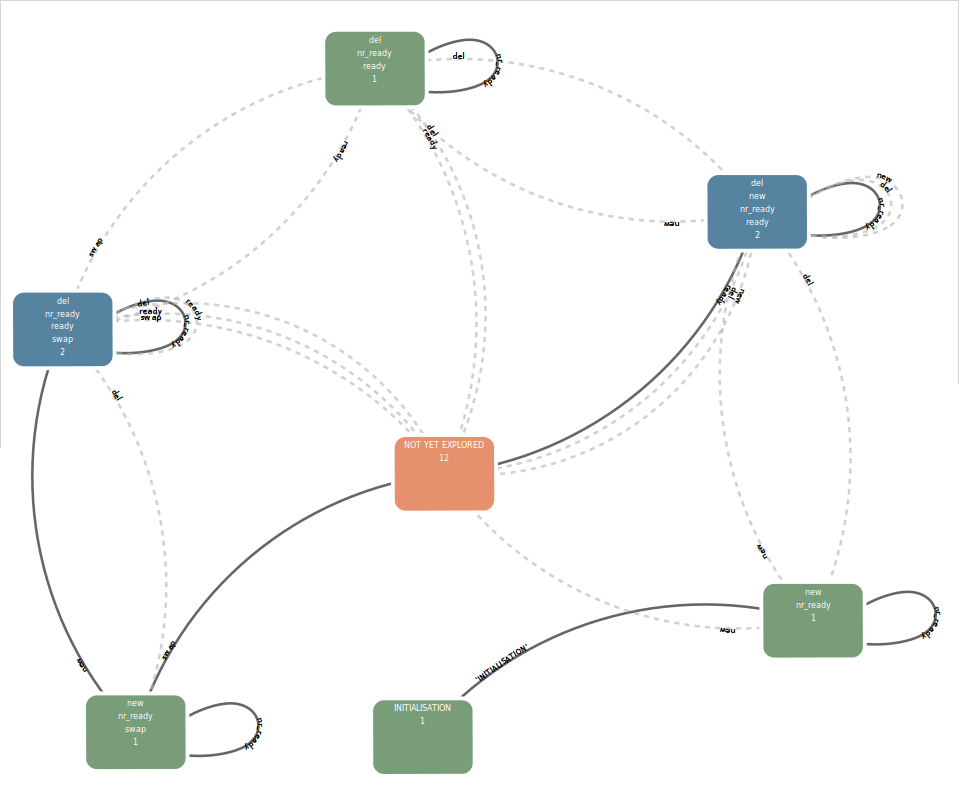
\includegraphics[width=15cm]{bilder/sigmerge.png}
\caption{D3 Visualization of signature merge for Scheduler example}
\label{sigmerge}
\end{figure}

\begin{figure}[h!]
\centering
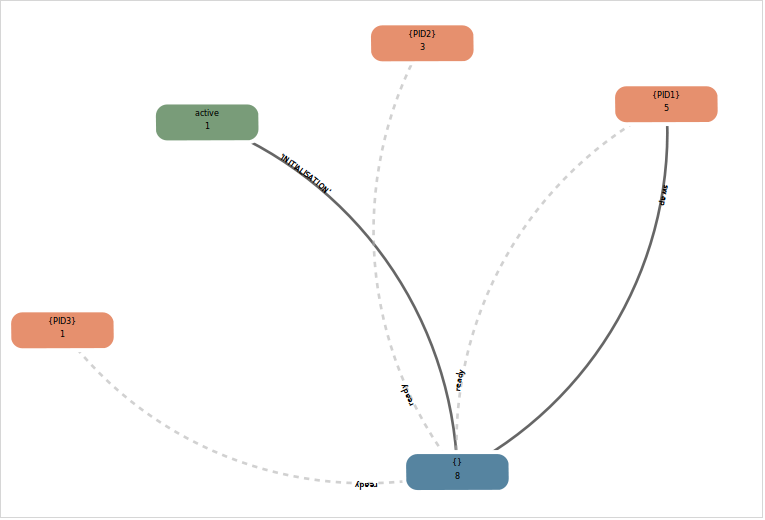
\includegraphics[width=15cm]{bilder/transdiag-wo.png}
\caption{D3 Visualization of the transition diagram of \texttt{active} in Scheduler example}
\label{transdiag}
\end{figure}

\begin{figure}[h!]
\centering
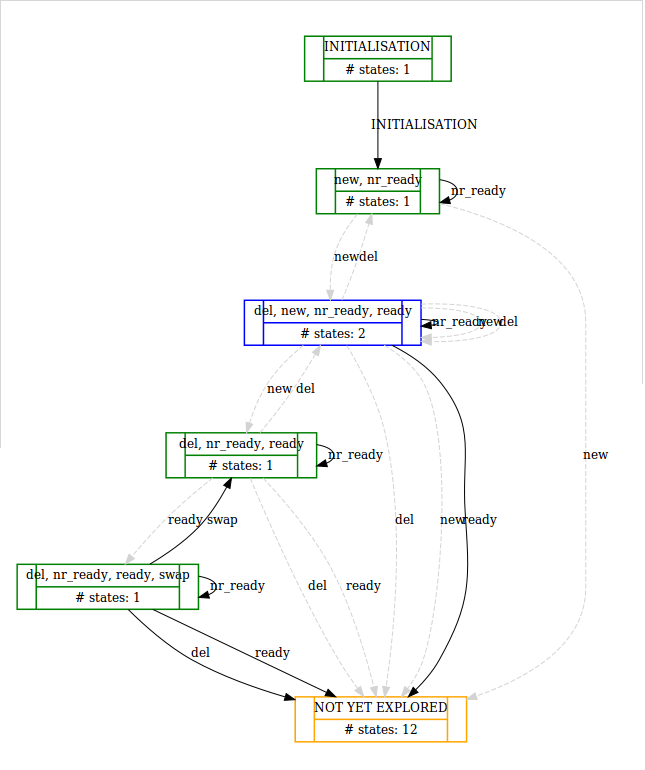
\includegraphics[width=15cm]{bilder/dotty-sigmerge.png}
\caption{Dotty Visualization of signature merge for the Scheduler example}
\label{sigmergeDotty}
\end{figure}

\begin{figure}[h!]
\centering
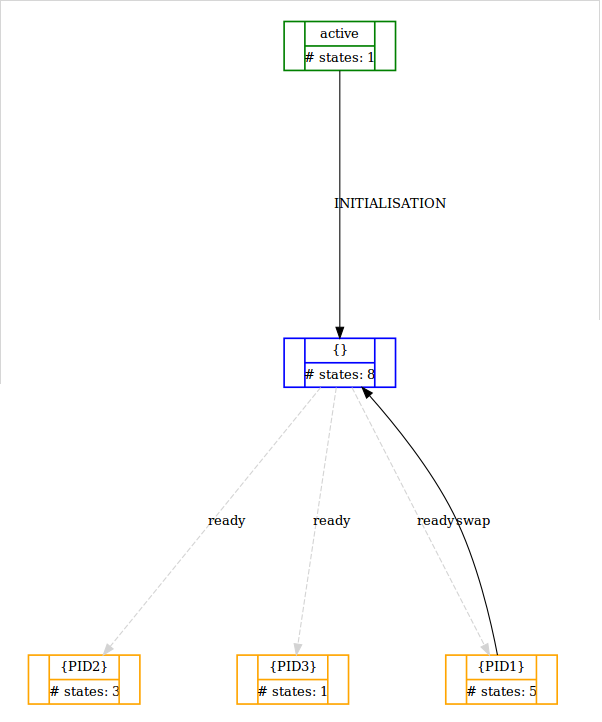
\includegraphics[width=15cm]{bilder/transdiag-dotty-wo.png}
\caption{Dotty Visualization of the transition diagram of \texttt{active} in Scheduler model}
\label{transdiagDotty}
\end{figure}

\subsubsection{UI} 
We also created the user interface.

\begin{figure}[h!]
\centering
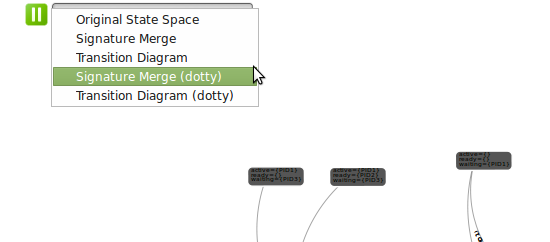
\includegraphics[width=15cm]{bilder/selectVisualization.png}
\caption{The user can select the desired visualization.}
\label{userSelect}
\end{figure}

\begin{figure}[h!]
\centering
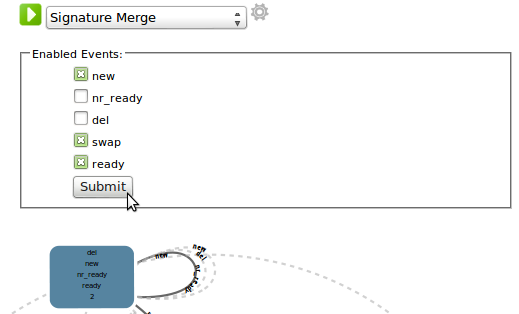
\includegraphics[width=15cm]{bilder/sigMergeUI.png}
\caption{User interface to chose events for signature merge.}
\label{sigMergeUI}
\end{figure}

\begin{figure}[h!]
\centering
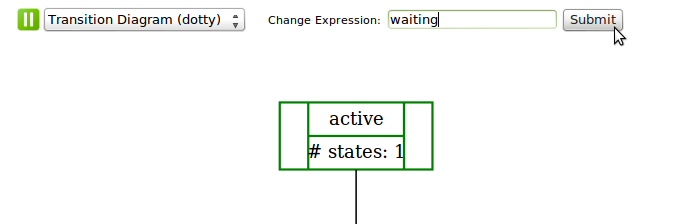
\includegraphics[width=15cm]{bilder/transDiag-UI.png}
\caption{The user can input a new expression to recalculate the transition diagram.}
\label{transDiagUI}
\end{figure}


\subsection{Visualization of a B-type Formula}

The ProB CLI already supported the functionality of expanding a formula into its subformulas and finding its value at a given state. However, the expanding of the formula took place lazily. A formula would be sent to the ProB CLI and then the direct subformulas of this formula would be sent back. The software would then have to contact ProB CLI recursively until all of the subformulas had been calculated and cached on the Java side. For the predicate visualization, we wanted the formula to be completely expanded and then sent in its entirety to the ProB 2.0 API. In order to do this, we implemented a prolog predicate within the ProB CLI that performs the recursive expanding of a B formula before it is sent back to the Java API. The predicate also delivers the value of each subformula for the given state. This ensures that performance will not an issue. 

The final visualization is interactive (\ref{predicate}). If a formula has subformulas, the user can select it from within the visualization to expand or to retract the subformulas. The subformulas are always either predicates or expressions. If they are expressions, they are colored white or light grey depending on whether they have subformulas or not. If the formula is a predicate that has evaluated to true for the given formula, the node is colored green. If the formula is a predicated that has evaluated to false, node is colored in red. The value of the given formula is also printed beneath the formula. This allows the user to visually identify the parts of the formulas and their given values. 

\begin{figure}[h!]
\centering
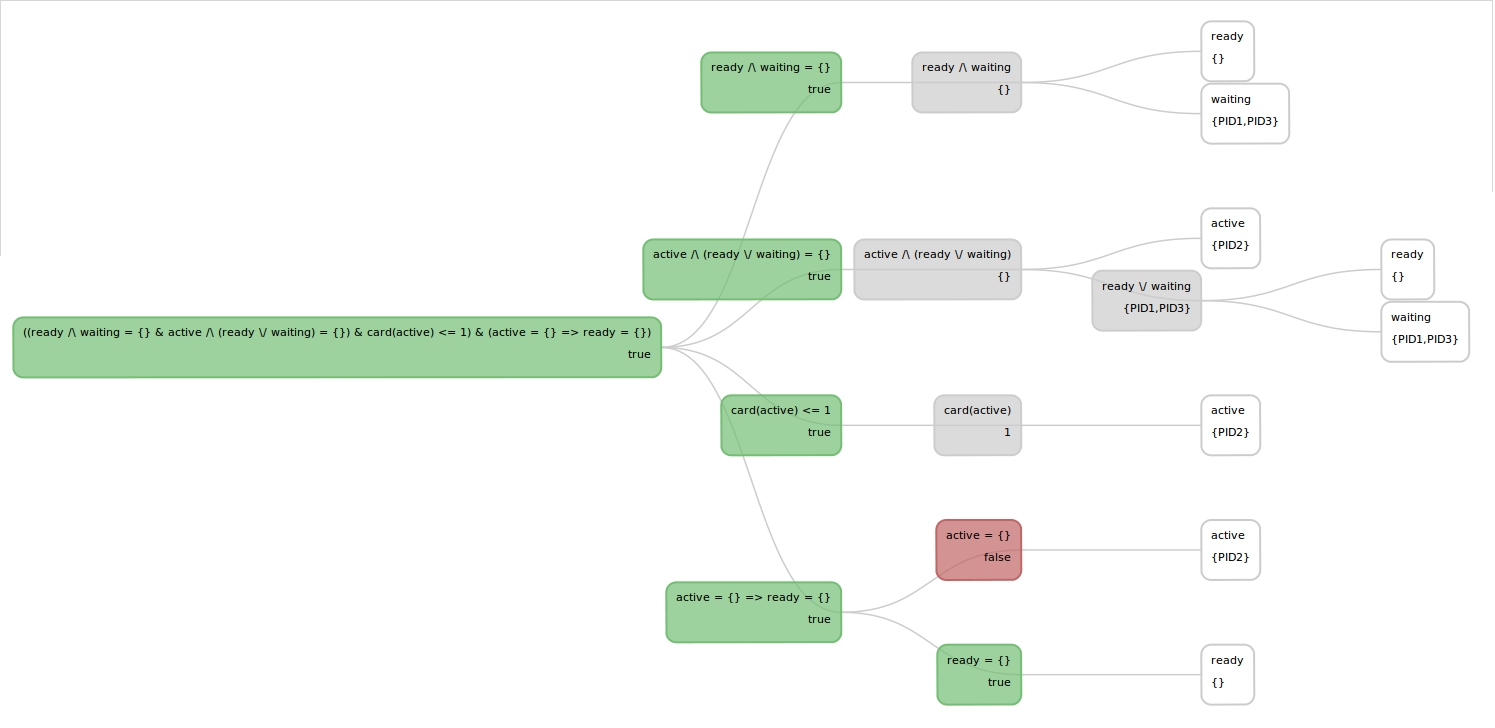
\includegraphics[width=15cm]{bilder/invariant.png}
\caption{Visualization of the invariant of the Scheduler model}
\label{predicate}
\end{figure}

In the implementation of the formula, the D3 tree layout is used. The expanding and collapsing of the nodes takes place with a simple JavaScript function. This visualization is based on the Collapsible Tree Layout from the D3 website (\ref{appendix:tree}). By harnessing the power of the D3 zoom behavior, it is also possible to zoom in and out of the visualization and to pan the image to inspect it closer. The servlet responsible for the visualization implements a listener to identify if any changes in the animation occur. If they do, the formula is recalculated for the new current state, and the visualization is redrawn.

\subsection{Visualization of the Value of a Formula Over Time}

The ProB 2.0 API supports the evaluation of a given formula over the course of the history of an animation.
Because a state is defined by the values that the variables take on when dealing with B type specification languages, it can be particularly interesting to be able to examine the value of a variable over the course of a trace when dealing with a Classical B or Event-B formula. 

In order for the ProB 2.0 API to evaluate a formula, it extracts the list of states that the animation visits over the course of its history. Then it contacts the ProB CLI and extracts the value that the formlua takes on for each state in the list. This information is then processed by D3 to produce a simple line plot (\ref{timeVsValue}). As of now, formulas can only be visualized if they take on integer values. In the future, we plan to support the visualization of formulas that take on boolean values. The visualization also interacts with the ProB 2.0 API. If the current state changes, the formula is recalculated and a new plot is produced.

\begin{figure}[h!]
\centering
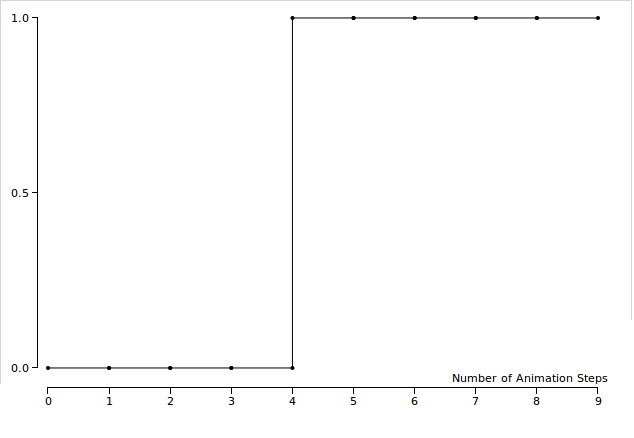
\includegraphics[width=15cm]{bilder/timeVsValue.png}
\caption{Visualization of value of \emph{card(active)} from the Scheduler model over the course of an animation.}
\label{timeVsValue}
\end{figure}

\subsection{Visualization framework}

One of the main issues that we had to be deal with at the beginning of the development process was the issue of how to integrate the visualizations into the ProB 2.0 API. At the time, the software already contained a functioning web server using Java servlets. Since the visualizations are written using Javascript and the d3 Javascript library, they needed to use the same framework. Because the visualizations needed to react to changes that take place during the animation of a model, they needed to be able to communicate with the ProB kernel. In order to accomplish this, a javascript function is invoked when the HTML page is loaded. This javascript sets up an interval so that the servlet that is responsible for the visualization is polled every 300 milliseconds to see if there are any changes. Both the servlet and the javascript function keep track of a counter that functions as a time stamp. This number is sent back and forth. If the javascript function identifies a discrepency between the numbers, it polls the servlet and then updates the visualization.

\begin{figure}[h!]
\centering
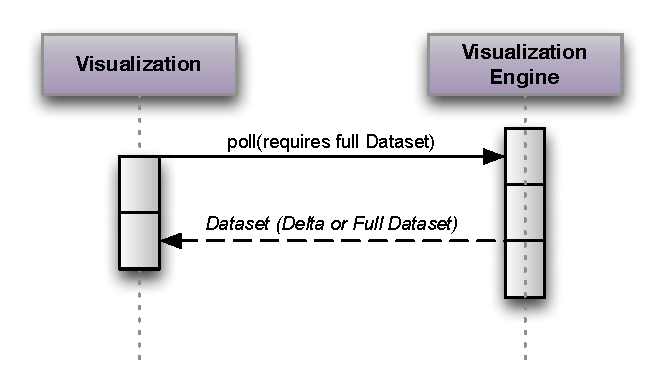
\includegraphics[width=15cm]{bilder/communication.pdf}
\caption{How visualizations communicate with the servlet that is responsible.}
\label{communication}
\end{figure}

\begin{figure}[h!]
\centering
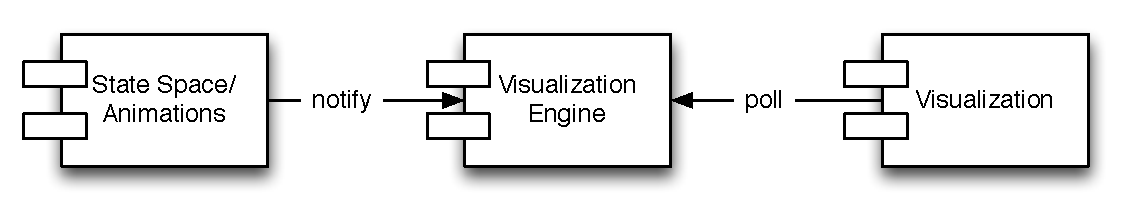
\includegraphics[width=15cm]{bilder/programFlow.pdf}
\caption{Model of the program flow.}
\label{programFlow}
\end{figure}

A problem quickly arose because the servlet is a singleton object. There is only one servlet responsible for all of the visualizations of a particular type. However, a static html page will always start with exactly the same values, and there is no good way for the javascript instances to determine what visualization they should belong to based on the content in the html page. The solution for this was to generate a unique session id and a servlet for every visualization. Using this id, an HTML page for the visualization is generated containing this unique identification number. When the HTML content is loaded, it calls the initialize function in the JavaScript script with the identification number as an id. The main servlet then uses the session id to determine which visualization servlet is responsible for the The JavaScript then sets up a polling interval and generates the visualization for the calculated data.

Once we implemented a way to integrate the visualization servlets into the ProB 2.0 application, it was still necessary to implement an easy way for the user to interact with the visualizations. One of the main advantages of the D3 visualization framework is the flexibility for the user. Using the D3 selectors, it is possible for the user to select and change the attributes of any of the elements of the visualization. In order to offer this functionality to the users from within the ProB 2.0 application, we decided that we needed to lift the functionality from the javascript level into the existing groovy console in the Java 2.0 API. This was accomplished by creating a \texttt{Transformer} object that represents the action that the user wants to carry out in the visualization. Then the \texttt{Transformer} object is added to the particular visualization and is applied the next time the visualization is redrawn. The \texttt{Transformer} object was written so that its functionality is similar to what the user would actually write using the D3 library.

We wanted how the user interacted with the visualization to be as natural as possible. The user should not have a hard time learning how to manipulate the visualization. For this reason, we decided to create a small DSL that would enable the user to specify which attributes should change within a particular visualization. It is possible for the user to create Transform objects in the console. This specifies a selection based on the W3C Selection API. It also specifies the attributes or styles that should be applied to the elements in question. Then this transformer is applied to a saved visualization.

\lstset{language=java}
\begin{lstlisting}[caption=Define rules for the transformation of visualization elements,label=tranformer]
// Select elements with ids "rroot" and "r1" and set their fill and stroke attributes
x = transform("#rroot,#r1") {
        set "fill", "red"
        set "stroke", "gray"
}

// Apply to visualization
viz0.apply(x)
\end{lstlisting}

It is also possible to harness the power of the Groovy closure in order to create a Transformer that can be parameterized.

\begin{lstlisting}[caption=Use Groovy closures to generate Transformers,label=transWclosure]
// Create a closure that can be parameterized
colorize = { selection, color ->
                transform(selection) {
                    set "fill",color
                }    
           }

// Color elements "rroot" and "r1" green
viz0.apply(colorize("#rroot,#r1","green"))
\end{lstlisting}

The ability to change visualizations in this way is built into all of the visualizations. It is therefore possible to manipulate all of the visualizations by changing the attributes that they contain.